\documentclass{article} % Класс печатного документа

% для поддержки русского языка
\usepackage[T2A]{fontenc} % поддержка специальных русских символов
\usepackage[utf8]{inputenc} % Кодировка исходного текста - utf8
\usepackage[english,russian]{babel} % Поддержка языка - русского с английским
\usepackage{indentfirst} % Отступ в первом абзаце

\usepackage{hyperref} % Для вставки гиперссылок
% \usepackage{listings} % Для вставки кусков кода
\usepackage{graphicx} % Вставка изображений
\usepackage{subfig} % Изображения друг напротив друга
\usepackage{float} % Для точного позиционирования картинок

% Default fixed font does not support bold face
\DeclareFixedFont{\ttb}{T1}{txtt}{bx}{n}{12} % for bold
\DeclareFixedFont{\ttm}{T1}{txtt}{m}{n}{12}  % for normal

% Custom colors
\usepackage{color}
\definecolor{deepblue}{rgb}{0,0,0.5}
\definecolor{deepred}{rgb}{0.6,0,0}
\definecolor{deepgreen}{rgb}{0,0.5,0}

\usepackage{listings}

% Python style for highlighting
\newcommand\pythonstyle{\lstset{
    language=Python,
    basicstyle=\ttm,
    otherkeywords={self},             % Add keywords here
    keywordstyle=\color{deepblue},
    emph={MyClass,__init__},          % Custom highlighting
    emphstyle=\color{deepred},    % Custom highlighting style
    stringstyle=\color{deepgreen},
    frame=tb,                         % Any extra options here
    showstringspaces=false,           % 
    basicstyle=\small,                % уменьшить размер шрифта
    columns=flexible                  % чтобы при копировании не было пробелов везде
}}


% Python environment
\lstnewenvironment{python}[1][]
{
\pythonstyle
\lstset{#1}
}
{}

% Python for external files
\newcommand\pythonexternal[2][]{{
\pythonstyle
\lstinputlisting[#1]{#2}}}

% Python for inline
\newcommand\pythoninline[1]{{\pythonstyle\lstinline!#1!}}

\makeatletter
\def\lst@outputspace{{\ifx\lst@bkgcolor\empty\color{white}\else\lst@bkgcolor\fi\lst@visiblespace}}
\makeatother
 % для красивого оформаления python кода

\title{Отчёт 8\protect\\
    Классификация.\\
    Метод бустинга бинарных деревьев решений (boosting)} % Заголовок документа
\author{Свичкарев А.\,В.} % Автор документа
\date{\today} % Текущая дата

\begin{document} % Конец преамбулы, начало текста

\maketitle % Печатает заголовок, список авторов и дату

\section{Цель}
Изучить способы решения задач классификации данных с
применением метода бустинга бинарных деревьев решений (Boosting).

\section{Задание №1}
Написать программу построения модели классификации синтетических данных
методом градиентного бустинга бинарных деревьев и визуализации деревьев решений.
Для формирования синтетических данных применить зависимость вида: $y = x + random$.
Построить и визуализировать частные модели деревьев, на основе которых методом
градиентного бустинга построить модель предсказания значений синтетических данных.
Привести значение минимального среднего квадрата ошибки Minimum MSE и график
зависимости среднего квадрата ошибок (mean squared error - MSE) от числа деревьев в
ансамбле и график предсказания значений синтетических данных.
\bigskip

Реализация на основе кода программы из Приложения (файл \verb$exercise1.py$):
\pythonexternal{../exercise1.py}
\bigskip

\clearpage
Примеры частных моделей деревьев глубины 5 не помещаются в отчёт,
поэтому прилагаются с отчётом.

\begin{figure}[H]
    \centering
    \noindent\makebox[\textwidth]{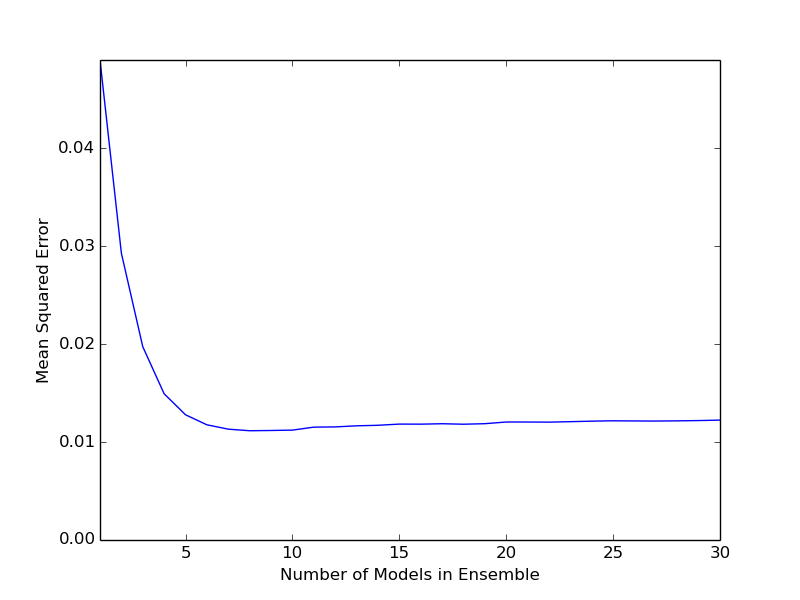
\includegraphics[width=0.6\paperwidth]{./mseEx1.png}}
    \caption{График зависимости среднего квадрата ошибок от числа деревьев в ансамбле}
\end{figure}
\bigskip

Значение минимального среднего квадрата ошибки Minimum MSE:
\lstinputlisting{./ex1_output.txt}

\begin{figure}[H]
    \centering
    \noindent\makebox[\textwidth]{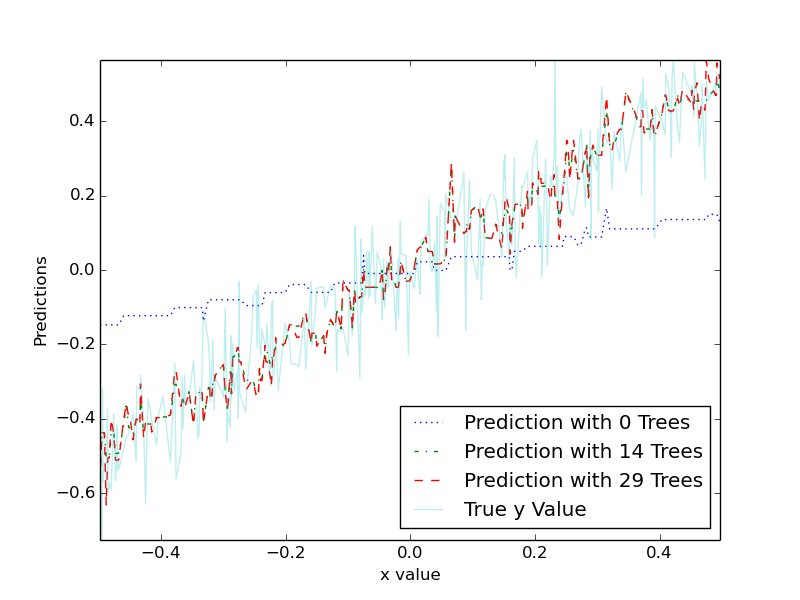
\includegraphics[width=0.6\paperwidth]{./predictionsEx1.png}}
    \caption{График предсказания значений синтетических данных в зависимости от числа деревьев в ансамбле}
\end{figure}
\bigskip

По графику MSE можно заметить, что уже при 7-8 деревьях в ансамбле достигается
минимальный для данной задачи результат. Впоследствие ошибка становится больше.

\clearpage
\section{Задание №2}
Выполнить классификацию синтетических данных методом градиентного бустинга бинарных
деревьев и визуализировать деревья решений.
Для формирования
синтетических данных применить зависимость вида: $y = a+b x^2 + random$. Привести
результаты предсказания значений синтетических данных.
\bigskip

Реализация на основе кода программы из Приложения (файл \verb$exercise2.py$):
\pythonexternal{../exercise2.py}
\bigskip

Примеры частных моделей деревьев глубины 5 не помещаются в отчёт,
поэтому прилагаются с отчётом.

\begin{figure}[H]
    \centering
    \noindent\makebox[\textwidth]{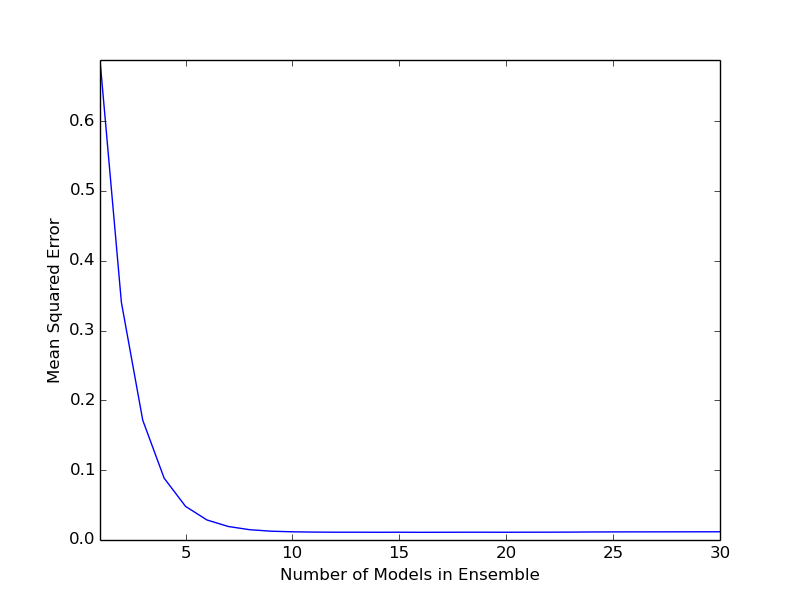
\includegraphics[width=0.6\paperwidth]{./mseEx2.png}}
    \caption{График зависимости среднего квадрата ошибок от числа деревьев в ансамбле}
\end{figure}
\bigskip

Значение минимального среднего квадрата ошибки Minimum MSE:
\lstinputlisting{./ex2_output.txt}

\begin{figure}[H]
    \centering
    \noindent\makebox[\textwidth]{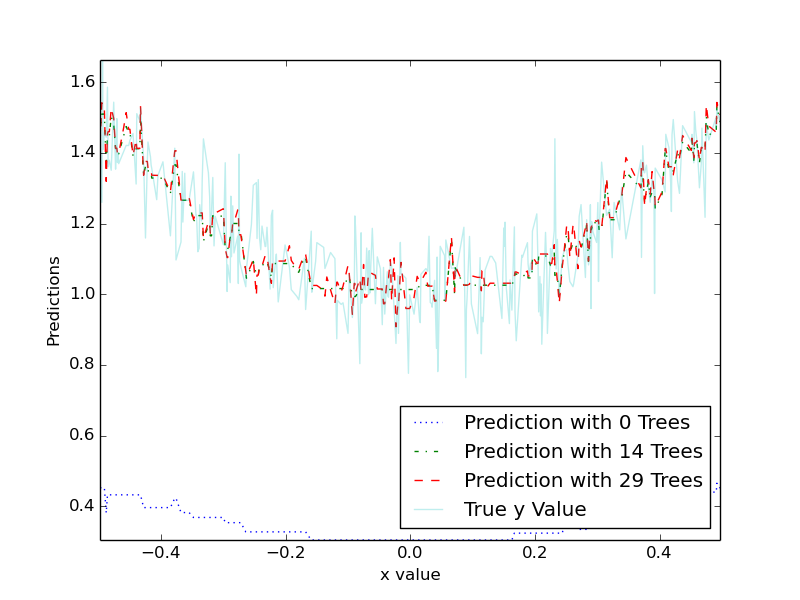
\includegraphics[width=0.6\paperwidth]{./predictionsEx2.png}}
    \caption{График предсказания значений синтетических данных в зависимости от числа деревьев в ансамбле}
\end{figure}
\bigskip

Метод бустинга схож с методом баггинга.
Данный метод показывает хорошие результаты для меньшей глубины деревьев,
так как в обучение следующих деревьев учитываются ошибки предыдущих,
таким образом результат уточняется. Однако у данного алгоритма есть
дополнительный параметр eps, от значения которого зависит скорость
достижения минимальной ошибки, если его не правильно подобрать,
то даже увеличение числа деревьев в ансамбле может не компенсировать возникающую ошибку.

\section{Пояснение}
Исходный код доступен по ссылке:
\href{https://github.com/SvichkarevAnatoly/Course-Python-Bioinformatics/tree/master/semester2/task8}
{github.com}

\end{document} % Конец документа
